\section*{Problem  Set 5}

\begin{mdframed}
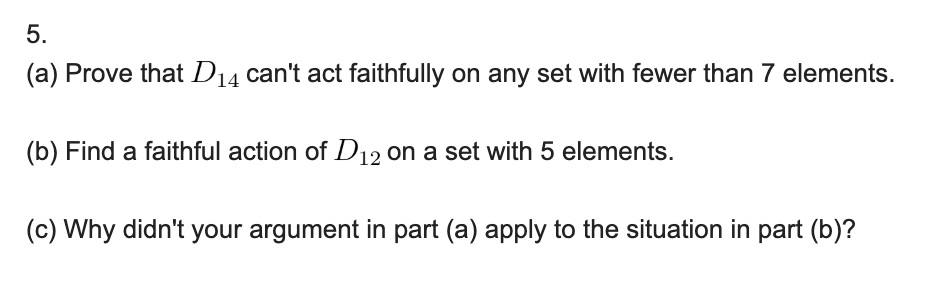
\includegraphics[width=400pt]{img/abstract-algebra--nf--4-1b73.png}
\end{mdframed}
{\bf (a)}
\begin{proof}
  $D_{14}$ is the group of $14$ symmetries of a regular heptagon.

  Suppose $\varphi: D_{14} \to S_A$ is a faithful action of $D_{14}$ on a set $A$.

\end{proof}



\begin{mdframed}
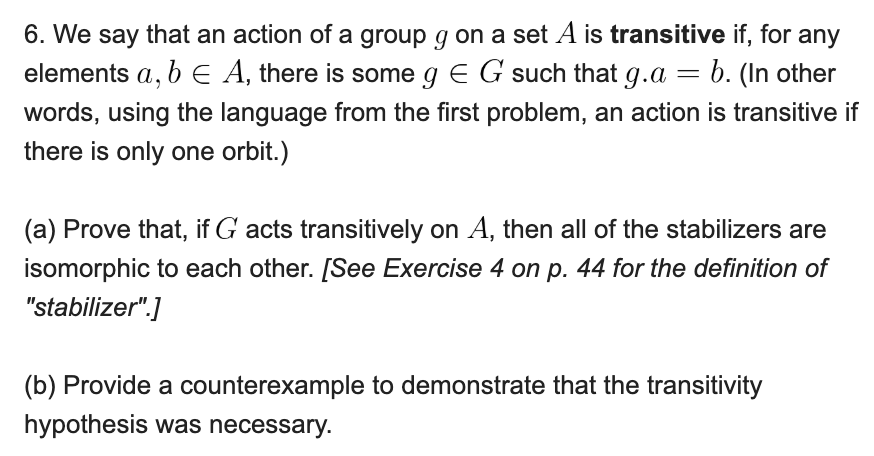
\includegraphics[width=400pt]{img/abstract-algebra--nf--4-50ae.png}
\end{mdframed}


\begin{mdframed}

\includegraphics[width=400pt]{img/abstract-algebra--nf--5-7356.png}
\end{mdframed}



\begin{mdframed}
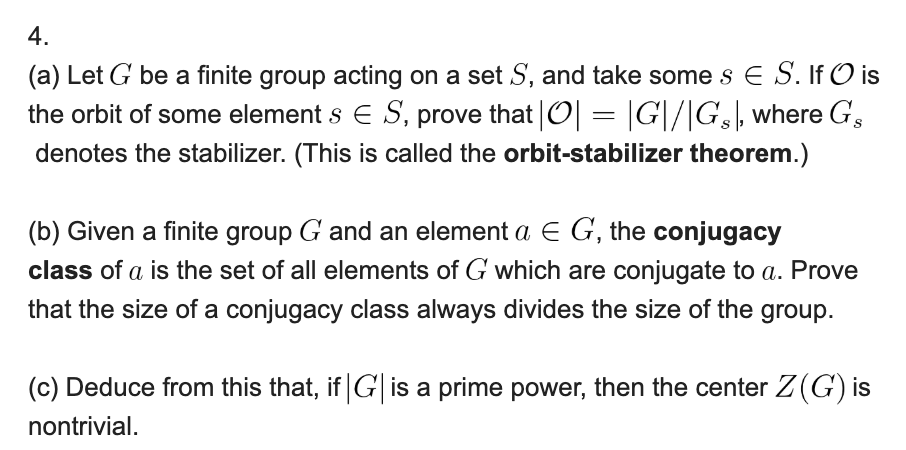
\includegraphics[width=400pt]{img/abstract-algebra--nf--5-23d3.png}
\end{mdframed}




\begin{mdframed}
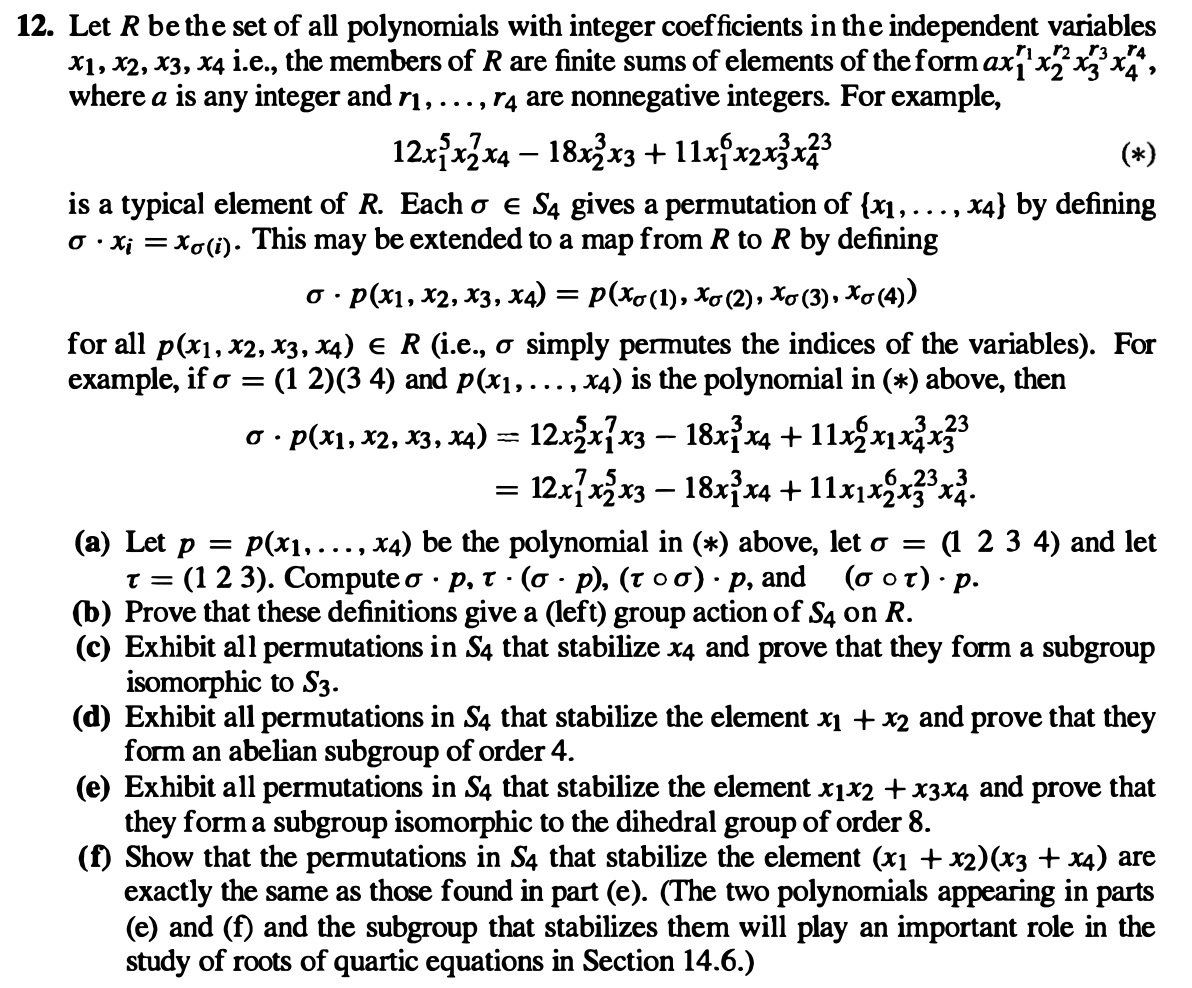
\includegraphics[width=400pt]{img/abstract-algebra--nf--5-4abb.png}
\end{mdframed}
